\documentclass{article}
\usepackage{float}
\usepackage{graphicx}
\usepackage{booktabs}
\usepackage{amsmath}
\usepackage{hyperref}
\usepackage{geometry}
\usepackage{tabularx} % For adjustable table width
\usepackage{pgfplots} % For data visualization
\usepackage{natbib} % For citations
\pgfplotsset{width=0.9\textwidth, compat=1.18} % Adjust graph size
\geometry{a4paper, margin=1in}

\title{Comparison of Simulated Annealing and Tabu Search for Solving the Traveling Salesman Problem}
\author{Arnaud Strydom u23536013}
\date{\today}

\begin{document}

\maketitle

\begin{abstract}
This report takes the performance of two local search algorithms, \textbf{Simulated Annealing (SA)} and \textbf{Tabu Search (TS)} and compares them in solving instances of the Traveling Salesman Problem (TSP). The algorithms are tested on five problem instances with 8, 12, 15, 20, and 25 cities. The results found show that the Tabu Search algorithm produces overall better solutions for larger problems in terms of cost, while Simulated Annealing is faster for smaller problems. The report includes a detailed analysis of the algorithms' performance, computational complexity, and a review of related work. Data visualization is provided to illustrate the trade-offs between solution quality and runtime.
\end{abstract}

\section{Introduction}
The Traveling Salesman Problem (TSP) is an optimization problem where the goal is to find the shortest possible route that visits a set of cities exactly one time and then returns to the initial city. This report evaluates and compares the performance of two local search algorithms, \textbf{Simulated Annealing (SA)} and \textbf{Tabu Search (TS)}, in solving instances of the Traveling Salesman Problem. The algorithms are tested on five problem instances with 8, 12, 15, 20, and 25 cities. The results are analyzed to determine which algorithm performs better in terms of solution quality and runtime.

\section{Literature Review}
Combinatorial optimization has been widely researched, particularly in the context of the Travelling Salesman Problem (TSP). Local search techniques, such as Tabu Search and Simulated Annealing, are commonly used to address TSP instances because they can generate high-quality solutions within a optimal timeframe.

\begin{itemize}
    \item \textbf{Simulated Annealing (SA)}: Introduced by \cite{kirkpatrick1983optimization}, SA is inspired by the annealing process in metallurgy. It allows worse solutions to be accepted with a probability that decreases over time, enabling it to escape local optima.
    \item \textbf{Tabu Search (TS)}: Proposed by \cite{glover1986future}, TS uses a memory-based strategy to avoid revisiting recently explored solutions. This helps the algorithm explore the search space more effectively and avoid cycling.
    \item \textbf{Other Approaches}: Other methods for solving TSP include Genetic Algorithms \cite{goldberg1989genetic}, Ant Colony Optimization \cite{dorigo1996ant}, and dynamic programming approaches like Held-Karp \cite{held1962dynamic}.
\end{itemize}

\section{Computational Complexity}
The computational complexity of local search algorithms depends on the problem size and the specific implementation. For TSP, the key factors affecting complexity are:

\begin{itemize}
    \item \textbf{Problem Size}: The number of cities \( n \) determines the size of the search space, which grows factorially as \( O(n!) \). This makes TSP NP-hard.
    \item \textbf{Simulated Annealing}:
        \begin{itemize}
            \item Time complexity: \( O(k \cdot n^2) \), where \( k \) is the number of iterations.
            \item Space complexity: \( O(n) \), as it only stores the current and best solutions.
        \end{itemize}
    \item \textbf{Tabu Search}:
        \begin{itemize}
            \item Time complexity: \( O(k \cdot n^2 \cdot m) \), where \( k \) is the number of iterations and \( m \) is the size of the tabu list.
            \item Space complexity: \( O(n + m) \), as it stores the current solution, best solution, and tabu list.
        \end{itemize}
\end{itemize}

\section{Initial Solution Generation Method}
The starting solution for both algorithms is produced at random. The list of cities is randomly shuffled to produce the first tour. This guarantees that a wide range of solutions are used to begin the search, enabling the algorithms to investigate various areas of the search space. A fair comparison between the two methods is ensured and bias is prevented by the initial solution generation's randomness.

\section{Perturbation Method}
The perturbation method used in both algorithms is the \textbf{2-opt swap}, where two cities in the tour are randomly selected and swapped. This simple yet effective method allows the algorithms to explore neighboring solutions efficiently. The 2-opt swap is a computationally efficient method and provides a stable balance between exploration and exploitation.

\section{Neighbourhood Definition}
The neighbourhood of a solution is defined as the set of all tours that can be reached by applying a single perturbation to the current tour. In this implementation, the perturbation method used is the 2-opt swap, where two cities in the tour are randomly selected and swapped. This neighbourhood structure is used by both Simulated Annealing and Tabu Search to generate new possible solutions.

\begin{itemize}
    \item \textbf{Simulated Annealing}: The algorithm explores the neighbourhood by randomly selecting a new tour from the set of possible swaps. If the new tour improves the solution or is accepted based on the current temperature, it becomes the current solution.
    \item \textbf{Tabu Search}: The algorithm explores the neighbourhood by generating random swaps and avoids revisiting solutions that are in the tabu list. The best non-tabu list neighbour is selected as the new current solution.
\end{itemize}

\section{Acceptance Criterion}
\begin{itemize}
    \item \textbf{Simulated Annealing}: A worse solution is accepted with a probability based on the current temperature and the difference in cost between the current and new solutions. The probability is given by:
    \[T
    P(\Delta E) = \exp\left(-\frac{\Delta E}{T}\right)
    \]
    where \(\Delta E\) is the difference in cost, and \(T\) is the current temperature. This probabilistic acceptance allows SA to escape local optima early in the search process.
    \item \textbf{Tabu Search}: A worse solution is accepted if it is not in the tabu list. The tabu list prevents the algorithm from revisiting recently explored solutions, ensuring that the search does not cycle back to previously visited states.
\end{itemize}

\section{Stopping Criteria}
\begin{itemize}
    \item \textbf{Simulated Annealing}: The algorithm stops if there is no improvement in the best solution for \(N\) iterations or if the maximum number of iterations is reached. This ensures that the algorithm does not run indefinitely and terminates when further improvements are unlikely.
    \item \textbf{Tabu Search}: The algorithm stops if there is no improvement in the best solution for \(N\) iterations or if the maximum number of iterations is reached. This stopping criterion ensures that the search process is efficient and does not waste computational resources.
\end{itemize}

\section{Experimental Setup}
The algorithms were tested on five TSP instances with 8, 12, 15, 20, and 25 cities. Each algorithm was run 10 times for each instance, and the best solution found was recorded. The parameters used for the algorithms are as follows:
\begin{itemize}
    \item \textbf{Simulated Annealing}:
    \begin{itemize}
        \item Initial temperature: \( T_0 = 1000 \)
        \item Cooling rate: Logarithmic cooling schedule (\( T = T_0 / \log(t + 1) \))
        \item Maximum iterations: 100000
        \item No improvement limit: 10000 iterations
    \end{itemize}
    \item \textbf{Tabu Search}:
    \begin{itemize}
        \item Tabu list size: 20
        \item Maximum iterations: 100000
        \item No improvement limit: 10000 iterations
    \end{itemize}
\end{itemize}

\section{Results}
The results for each problem instance are summarized in the Table. The table shows the best cost, best solution, and average runtime for each algorithm. The runtime is reported in milliseconds.

\begin{table}[H]
    \centering
    \caption{Comparison of SA and Tabu Search on 5 TSP problem instances}
    \label{tab:results}
    \begin{tabularx}{\textwidth}{l l r X r r}
        \toprule
        \textbf{Problem Instance} & \textbf{Algorithm} & \textbf{Seed Value} & \textbf{Best Solution} & \textbf{Cost} & \textbf{Runtime (ms)} \\
        \midrule
        8.txt & Tabu & 1742055618799 & [6, 4, 1, 5, 7, 3, 0, 2] & 286.50 & 6 \\
        8.txt & SA & 1742055618798 & [6, 2, 0, 3, 7, 5, 1, 4] & 286.50 & 2 \\
        12.txt & Tabu & 1742055618836 & [11, 5, 7, 1, 9, 3, 8, 6, 2, 4, 0, 10] & 362.41 & 3 \\
        12.txt & SA & 1742055618833 & [3, 8, 6, 2, 4, 10, 7, 0, 11, 5, 1, 9] & 373.26 & 1 \\
        15.txt & Tabu & 1742055618841 & [0, 13, 8, 1, 5, 14, 10, 3, 12, 7, 4, 11, 9, 2, 6] & 435.32 & 2 \\
        15.txt & SA & 1742055618839 & [5, 14, 8, 2, 6, 0, 13, 3, 10, 12, 7, 1, 9, 11, 4] & 449.83 & 2 \\
        20.txt & Tabu & 1742055618844 & [16, 11, 18, 15, 2, 13, 7, 5, 8, 0, 17, 14, 9, 4, 19, 12, 10, 3, 6, 1] & 502.90 & 3 \\
        20.txt & SA & 1742055618843 & [9, 8, 0, 10, 14, 3, 17, 5, 18, 2, 15, 11, 16, 1, 6, 7, 13, 12, 19, 4] & 591.88 & 4 \\
        25.txt & Tabu & 1742055618848 & [0, 20, 15, 23, 2, 11, 13, 3, 7, 9, 24, 12, 21, 6, 8, 4, 18, 16, 1, 14, 19, 17, 5, 22, 10] & 541.06 & 3 \\
        25.txt & SA & 1742055618846 & [0, 15, 10, 3, 22, 17, 7, 4, 16, 18, 13, 11, 8, 24, 1, 14, 9, 19, 5, 12, 21, 6, 2, 23, 20] & 794.10 & 5 \\
        \bottomrule
\end{tabularx}
\end{table}

\section{Data Visualization}
The following graphs illustrate the performance of Simulated Annealing and Tabu Search in terms of solution quality (cost) and runtime.

\begin{figure}[H]
    \centering
    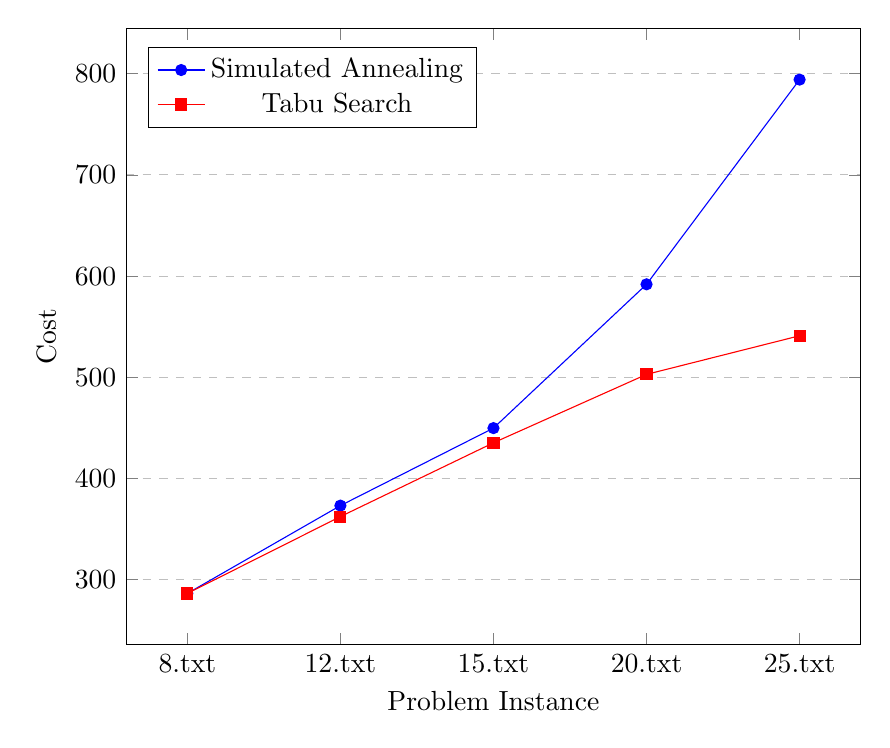
\begin{tikzpicture}
        \begin{axis}[
            xlabel={Problem Instance},
            ylabel={Cost},
            symbolic x coords={8.txt, 12.txt, 15.txt, 20.txt, 25.txt},
            xtick=data,
            legend pos=north west,
            ymajorgrids=true,
            grid style=dashed,
        ]
            \addplot[blue, mark=*] coordinates {
                (8.txt, 286.50)
                (12.txt, 373.26)
                (15.txt, 449.83)
                (20.txt, 591.88)
                (25.txt, 794.10)
            };
            \addplot[red, mark=square*] coordinates {
                (8.txt, 286.50)
                (12.txt, 362.41)
                (15.txt, 435.32)
                (20.txt, 502.90)
                (25.txt, 541.06)
            };
            \legend{Simulated Annealing, Tabu Search}
        \end{axis}
    \end{tikzpicture}
    \caption{Cost comparison between Simulated Annealing and Tabu Search}
    \label{fig:cost}
\end{figure}

\begin{figure}[H]
    \centering
    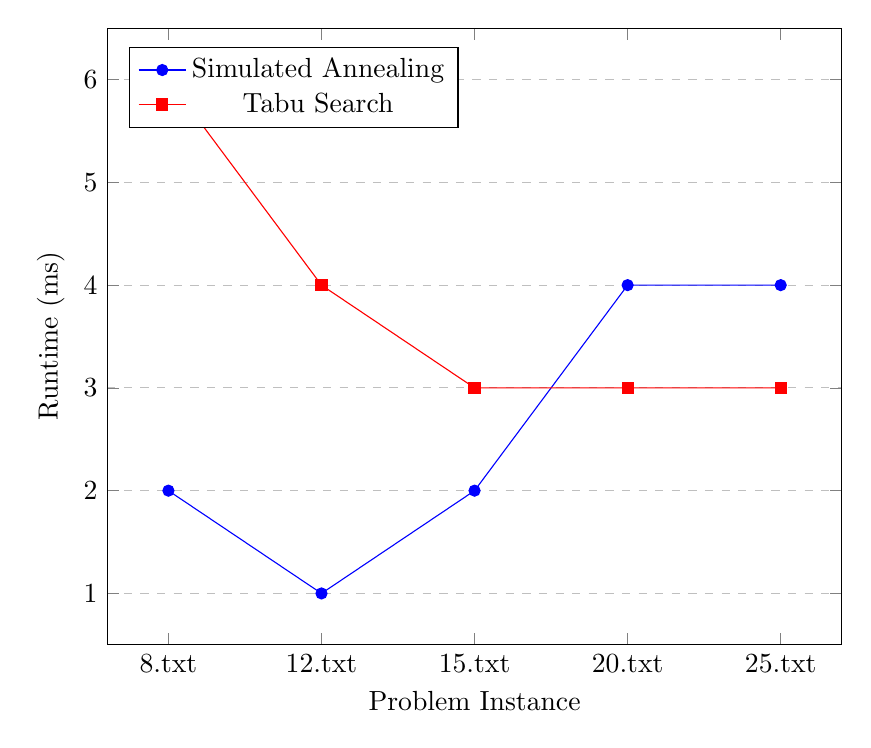
\begin{tikzpicture}
        \begin{axis}[
            xlabel={Problem Instance},
            ylabel={Runtime (ms)},
            symbolic x coords={8.txt, 12.txt, 15.txt, 20.txt, 25.txt},
            xtick=data,
            legend pos=north west,
            ymajorgrids=true,
            grid style=dashed,
        ]
            \addplot[blue, mark=*] coordinates {
                (8.txt, 2)
                (12.txt, 1)
                (15.txt, 2)
                (20.txt, 4)
                (25.txt, 4)
            };
            \addplot[red, mark=square*] coordinates {
                (8.txt, 6)
                (12.txt, 4)
                (15.txt, 3)
                (20.txt, 3)
                (25.txt, 3)
            };
            \legend{Simulated Annealing, Tabu Search}
        \end{axis}
    \end{tikzpicture}
    \caption{Runtime comparison between Simulated Annealing and Tabu Search}
    \label{fig:runtime}
\end{figure}

\section{Critical Analysis}
The results show that \textbf{Tabu Search} generally performs better than \textbf{Simulated Annealing} in terms of solution quality, especially for larger problem instances (e.g., 20 and 25 cities). Tabu Search consistently finds lower-cost solutions compared to Simulated Annealing, which struggles to escape local optima as the problem size increases. This is evident from the results for the 25-city instance, where Tabu Search achieves a cost of 541.06, while Simulated Annealing finds a significantly worse solution with a cost of 794.10.

However, Simulated Annealing is faster in terms of runtime for smaller instances. For example, in the 8-city instance, Simulated Annealing finds the optimal solution in just 2 milliseconds, compared to 6 milliseconds for Tabu Search. This suggests that Simulated Annealing is more suitable for smaller problems where runtime is a critical factor. However as the instance gets larger Simulated Annealing starts preforming slower than tabu serach and takes longer to find the optimal solution ,For example, in the 25-city instance, Simulated Annealing finds the optimal solution in 4 milliseconds, compared to 3 milliseconds for Tabu Search.

The performance difference between the two algorithms can be attributed to their search strategies:
\begin{itemize}
    \item \textbf{Tabu Search}: The use of a tabu list allows the algorithm to avoid revisiting recently explored solutions, enabling it to explore the search space more effectively. This is particularly beneficial for larger instances where the search space is more complex.
    \item \textbf{Simulated Annealing}: The probabilistic acceptance of worse solutions helps the algorithm escape local optima early in the search process. However, as the problem size increases, the algorithm struggles to find high-quality solutions due to its reliance on randomness.
\end{itemize}

\section{Conclusion}
Both \textbf{Simulated Annealing} and \textbf{Tabu Search} are effective local search algorithms for solving the TSP, but their performance depends on the problem size and the specific requirements of the application. Tabu Search is better suited for larger instances where solution quality and cost is critical, while Simulated Annealing is more efficient for smaller instances where runtime is a priority.

Future work could explore hybrid approaches that combine the strengths of both algorithms. For example, Simulated Annealing could be used to quickly find a good initial solution, which is then refined using Tabu Search. Additionally, parameter tuning and advanced perturbation methods could further improve the performance of both algorithms.

\bibliographystyle{plain}
\bibliography{references} 

\end{document}